\chapter{Implementation}
\label{ch:impl}

The system was built in two iterations. Iteration~1 ran from the start of the project to the mid evaluation on 21 October 2026 and produced the vision prototype and the first web application. Iteration~2 ran from the mid evaluation to the submission of this report and turned the prototype into a connected system: a shared database, the event store, the agents, dispatch, the dashboard binding and security hardening. All code is in the repository \path{muhammad-moiz-ansari/retail-store-analysis}; this report describes the \path{fyp2-moiz} branch at commit \texttt{c8ff409} (26 November 2026).

\section{Technology Stack}
\begin{table}[H]
\centering
\caption{Technology stack}\label{tab:stack}
\begin{tabular}{P{0.2\textwidth}P{0.42\textwidth}P{0.3\textwidth}}
\toprule
Layer & Technology & Why\\
\midrule
Vision & Python 3.11, Ultralytics YOLOv8n and YOLOv8n-pose, OpenVINO, BoT-SORT, OpenCV & Small models that run on a CPU; OpenVINO speeds up CPU inference\\
Backend & FastAPI on Uvicorn, Pydantic contracts & Typed request and result models that reject malformed data\\
Agents & LangGraph state graph, five typed read-only tools & Explicit, testable control flow; no free database access\\
Database & PostgreSQL 17 (Neon for the hosted instance), psycopg 3 & One database for application, event and identity data\\
Web & Next.js 15, React 19, TypeScript, Recharts & Server-side session handling and a proxy that keeps secrets off the browser\\
Testing & pytest, Node test runner, GitHub Actions & Three CI jobs on every push\\
Optional services & Hugging Face inference router, ElevenLabs & Question routing and spoken task instructions\\
\bottomrule
\end{tabular}
\end{table}

\section{Iteration 1: Vision Prototype and Web Application}
Iteration~1 established the pieces later work builds on.
\begin{itemize}
\item \textbf{Dataset.} The team recorded its own footage because retailers would not share theirs; the supervisor accepted the resulting 70-video dataset on 12 October 2026. A role detector (\path{best.pt}) was trained on customer and employee classes.
\item \textbf{Interaction pipeline.} Body-height-normalised proximity nominated employee--customer pairs, a pass-by filter rejected people walking past, and a YOLO pose judge checked whether heads faced each other. On the one labelled clip available then, the judge removed the only false positive.
\item \textbf{Web application.} A Next.js application with manager and employee pages, signed session cookies and an internal secret on backend calls.
\item \textbf{Descoped floor prototype.} A calibrated floor-distance prototype projected foot points into metres. The moving-camera footage produced almost no valid projections, so it was descoped in favour of body-height distance.
\end{itemize}
The mid evaluation found the report's figures and requirements incorrect. Iteration~2 therefore included rebuilding both, which this report presents.

\section{Iteration 2: From Prototype to Connected System}

\subsection{Model Consolidation}
Tests on corridor footage showed that the store-trained role detector missed clearly visible people (it found 53--56 of the 140 people that the COCO model found), because it had only seen the team's store. The pipeline now uses the COCO YOLOv8n model to find and track everyone, and runs the role detector only to label each new track during its first second, rechecking every two seconds. When every visible track already has a fresh label, the role detector does not run at all, which saves CPU time.

\subsection{Labelling and Evaluation Tooling}
Twenty-five clips were labelled in CVAT with interaction intervals, pass-bys and reviewed person roles, and imported with \path{cvat_import.py}. A benchmark command scores detector, interaction, role, tracking and speed results; a confidence command adds bootstrap intervals; and a refit command fits role weights with leave-one-clip-out validation. Chapter~\ref{ch:cveval} reports the results.

\subsection{Event Store and PostgreSQL}
Every run is converted by \path{backend/events/ingest.py} into the ten event tables of Table~\ref{tab:event-tables}. Ingestion derives unattended episodes (a customer who waits past the store's threshold without a \emph{confirmed} interaction), per-minute camera health, hourly heatmaps and, for an entrance camera, directional footfall with hysteresis so that a person hovering on the line is counted once. A synthetic fixture day\label{sec:fixture} with planted patterns (an evening rush, an understaffed aisle and a blocked camera) lets every later layer be tested before real footage is stored.

On 11 November 2026 the application moved from SQLite to PostgreSQL, so that accounts, events and camera identities share one database. Analytics reads run in read-only, repeatable-read transactions, and legacy SQLite data can be imported in one transaction with identifiers and password hashes preserved. Ingestion is currently a command run after a job; triggering it automatically when a web-started job finishes is FYP-2 work.

\subsection{Agent Layer}
The agent layer was built in four steps:
\begin{enumerate}
\item \textbf{Typed contracts and five read-only tools} (footfall, zone dwell, interactions, unattended episodes, coverage). Each result carries its time window, filters, evidence references and limitations, and returns \emph{unavailable} rather than zero when its source is missing.
\item \textbf{A scoped registry} that binds tools to the caller's store and allowed runs, cameras and zones, and rejects any attempt to override them in the tool arguments.
\item \textbf{The orchestration graph} (Figure~\ref{fig:graph}) with routing, grounding, one repair and development traces. The router can optionally ask a language model which agent should answer; the model sees only the question and cannot choose tools or supply figures.
\item \textbf{Two business agents.} The Customer Behavior agent answers questions about traffic, dwell, interactions and waiting customers; the Employee Activity agent answers questions about staff coverage and assistance. Both are registered as real agents, not development stubs, and build their answers only from claims that point at tool metrics.
\end{enumerate}
On top of these, the \emph{Insight Narration} digest assembles traffic, assistance, waiting-customer and coverage sections from verified claims, and a narrative check rejects any text that contains a number not backed by a claim. A clip-review module prepares 10--20\,s review clips for each event, in a blind mode that hides the system's verdict, and computes precision and Cohen's kappa once two reviewers have recorded their verdicts.

\subsection{Occupancy Categories and Map Registration}
Following the team's decision of 11 November 2026, live occupancy uses exactly four categories for an observed map cell: \emph{customer}, \emph{employee}, \emph{customer and employee}, and \emph{no one}. A cell whose camera coverage or role evidence is insufficient is masked with a quality reason instead of being given a category, so a blocked camera is never shown as an empty area. A tracker applies hysteresis so a category changes only after it holds for two consecutive windows. Map registration (\path{backend/events/spatial.py}) projects foot points onto a supplied floor map and writes per-cell dwell; it has been tested on synthetic geometry only, because the store's floor plan and camera calibration points have not yet been supplied. Separately, the Interactions page shows a per-camera attention state (hot, gray, green or inactive) from the customer-to-employee ratio; it is an indicator on the live video, not a fifth category.

\subsection{Signal Policy and Dispatch}
The signal policy turns a closed window into at most one unattended-customer and one unstaffed-zone decision per zone, each with a reason code. Its thresholds are store configuration: by default a customer must wait 180\,s, a wait of 360\,s or three waiting customers makes the event high priority, a zone is short of staff below a 25\,\% staffed share, and both events are suppressed when more than 20\,\% of the window was unobserved. Synthetic evidence never dispatches a real task unless a demo flag is set.

The dispatch handler selects an eligible employee: active, rostered, available, without an open task and not currently in an interaction, and only if taking them keeps their own zone at its minimum staff. It ranks staff of the target zone first, then floaters, then the zone with the most spare staff, and writes the event, alert, task, task event and decision in one transaction. A unique key on the event makes repeats return the earlier decision. The employee page receives new tasks through a server-sent event stream, and a spoken version of the instruction is generated on demand, falling back to the browser's own speech when no provider key is configured.

\subsection{Dashboard and Web Application}
The dashboard reads through a typed provider that validates every payload, shows eight aggregate metrics with units, evidence and limitations, and distinguishes loading, observed-empty, partial, unavailable and stale states. Its default source is the configured backend; synthetic preview data is available only when explicitly chosen and is labelled on screen. Backend dashboard routes check that the signed-in manager is active and a member of the store before reading anything. The dashboard also hosts the Ask panel, a list of recent interaction events without track identities, and a System Status view of dispatch outcomes and acknowledgement times.

\subsection{Aisle Relay Demonstration}
To show the whole loop on video, a demonstration splits one recorded clip into two aisles (left: Aisle~1, right: Aisle~2), runs one tracking pass, and treats an aisle with customers and no employee as a staffing need. The resulting alert and task reach a signed-in employee's home page; when an employee is later seen in that aisle, the task completes and the alert resolves with the camera recorded as the actor. The two aisles are halves of one recording, so this is a demonstration of the flow, not an evaluation of multi-camera handoff.

\subsection{Security Hardening}
A code review in November 2026 found ten issues (Table~\ref{tab:security}); every actionable one was fixed and covered by tests.

\begin{table}[H]
\centering
\caption{Security review findings and fixes}\label{tab:security}
\begin{tabular}{P{0.06\textwidth}P{0.12\textwidth}P{0.37\textwidth}P{0.35\textwidth}}
\toprule
ID & Severity & Finding & Fix\\
\midrule
S1 & High & Secrets fell back to fixed defaults when unset & Backend and web tier refuse to start or serve with missing or default secrets outside development\\
S2 & Medium & Internal secret compared with \texttt{!=} & Constant-time comparison\\
S3 & Medium & No sign-in rate limit & Account lock after 5 failures in 15 min; address limit of 20; Ask limited to 10 per minute per manager\\
S4 & Medium & Backend trusts actor headers after the secret check & Secret kept server-side; proxy strips browser-supplied actor headers\\
S5 & Low & PBKDF2 with 120\,000 iterations & 600\,000 iterations~\cite{owaspPasswords}; old hashes upgraded at next sign-in\\
S6 & Low & Minimum password length 6 & Minimum 8\\
S7 & Low & Invitation tokens stored in plain text & Stored as SHA-256 hashes\\
S8 & Low & Unbounded CV jobs & At most 2 running jobs; last 50 finished kept\\
-- & High & Employees could reach camera routes & Every camera route except health now requires the Manager role\\
\bottomrule
\end{tabular}
\end{table}

\subsection{Continuous Integration}
A GitHub Actions workflow runs three jobs on every push: a fast backend job against a PostgreSQL 17 service, a frontend job (lint, type check, provider tests and production build), and the slow vision suite. All three passed on the integration branch \path{fyp-2} (workflow run \#24, commit \texttt{fd048f0}).

\section{User Interface}
\label{sec:ui}
The screenshots in this section were captured on 26 November 2026 from the system at commit \texttt{c8ff409}, running locally against a PostgreSQL database loaded with the synthetic fixture day (Section~\ref{sec:fixture}) and one staffing task dispatched by the real operations path. Every figure shown comes from the backend; where the data is synthetic, the interface says so itself. The pages are shown in the order a manager and an employee use them.

\begin{figure}[htbp]
\centering
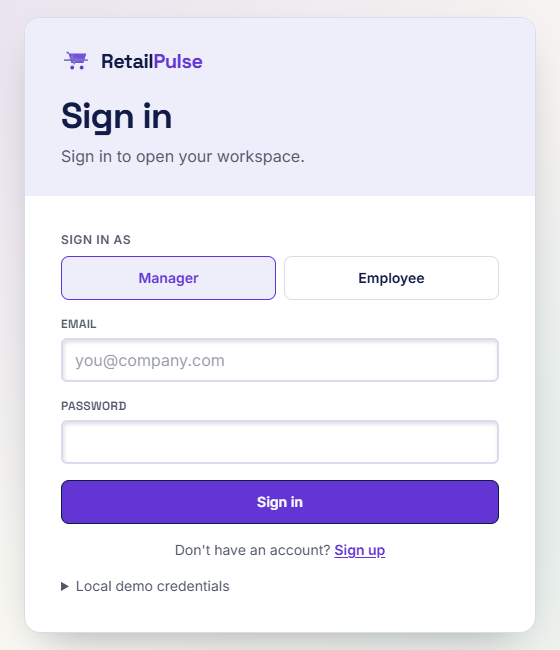
\includegraphics[width=0.42\textwidth]{ThesisFigs/ui_login.png}
\caption[Sign-in page]{Sign-in page. The user chooses the Manager or Employee workspace; a choice that does not match the stored role is refused (FR-02).}
\label{fig:ui-login}
\end{figure}

\begin{figure}[htbp]
\centering
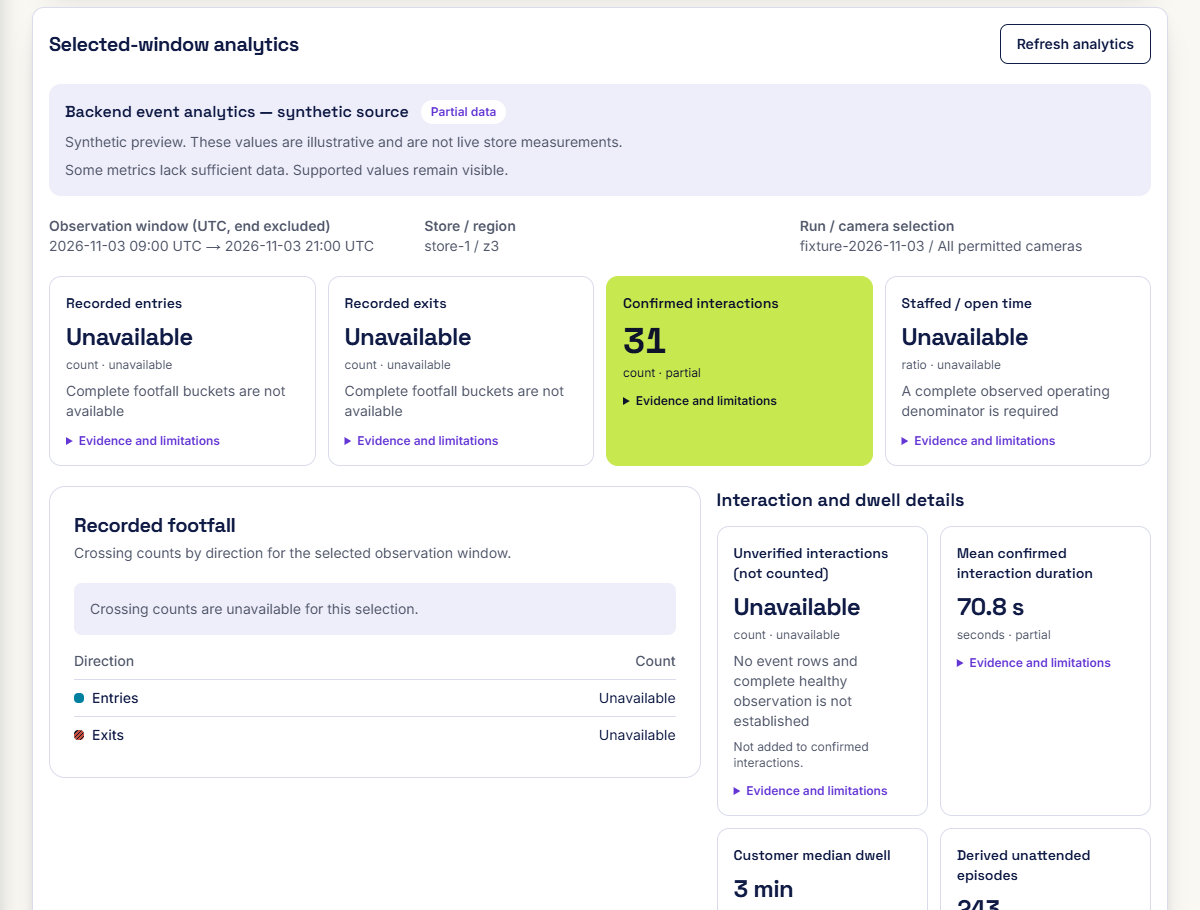
\includegraphics[width=\textwidth]{ThesisFigs/ui_dashboard.png}
\caption[Manager dashboard]{Manager dashboard for aisle z3 over the fixture day. The banner marks the source as synthetic and the data as partial; metrics without enough evidence (footfall, staffed share) are shown as unavailable with the reason rather than as zero (FR-17, NFR-06).}
\label{fig:ui-dashboard}
\end{figure}

\begin{figure}[htbp]
\centering
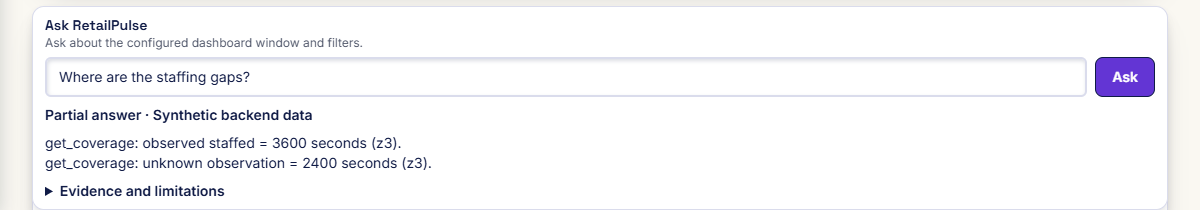
\includegraphics[width=\textwidth]{ThesisFigs/ui_ask.png}
\caption[Ask panel answering a staffing question]{Ask panel answering ``Where are the staffing gaps?''. Each line names the tool and metric it came from; the answer is marked partial because 2\,400 of the zone's seconds were unobserved (FR-18, FR-19).}
\label{fig:ui-ask}
\end{figure}

\begin{figure}[htbp]
\centering
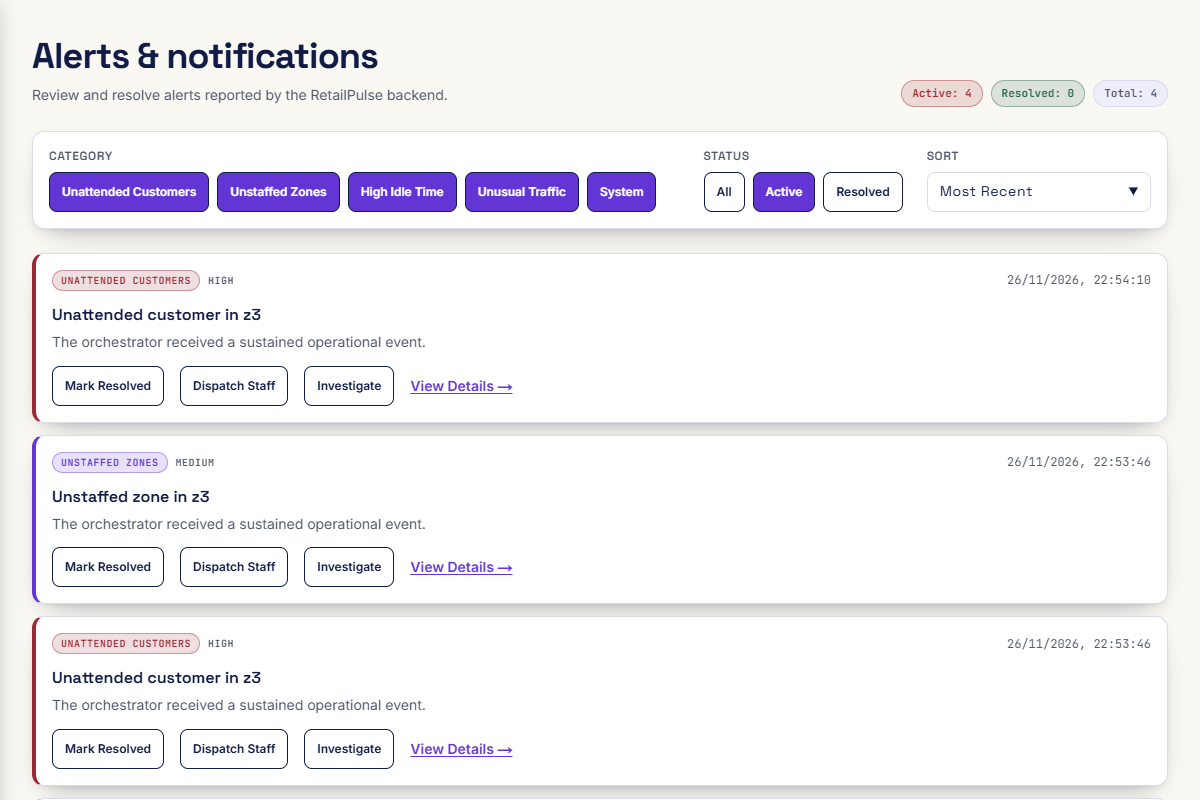
\includegraphics[width=\textwidth]{ThesisFigs/ui_alerts.png}
\caption[Alerts page]{Alerts page with the unattended-customer and unstaffed-zone events raised for aisle z3, filters by category and status, and actions to resolve, dispatch or investigate (FR-30).}
\label{fig:ui-alerts}
\end{figure}

\begin{figure}[htbp]
\centering
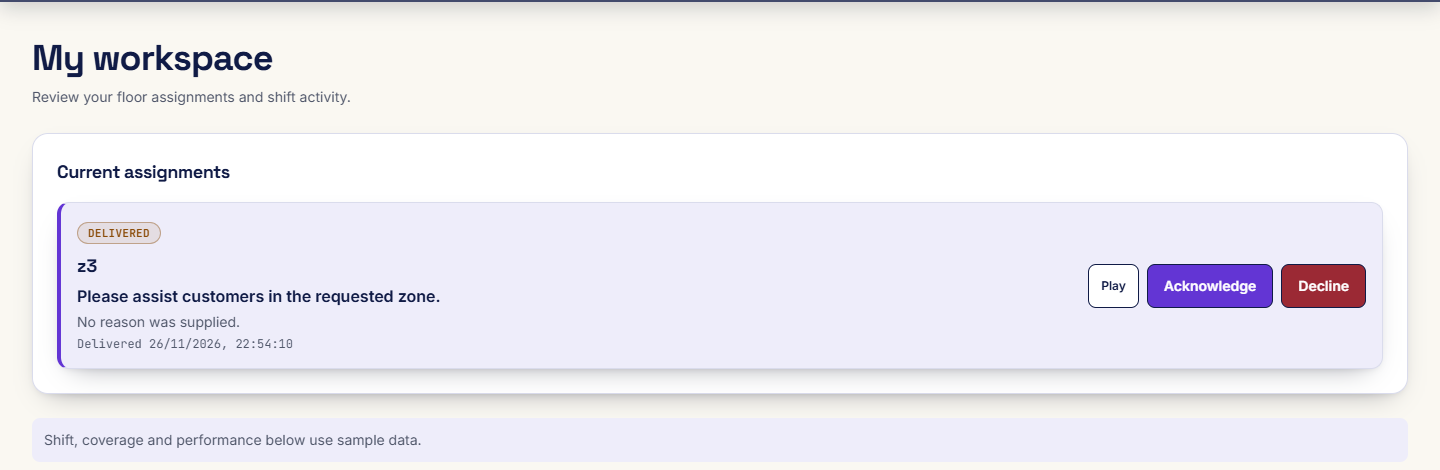
\includegraphics[width=\textwidth]{ThesisFigs/ui_employee_home.png}
\caption[Employee workspace with a dispatched task]{Employee workspace showing the task dispatched for aisle z3 in the \emph{delivered} state, with Play (spoken instruction), Acknowledge and Decline (FR-27 to FR-29). The shift cards below it use sample data and are labelled as such on the page.}
\label{fig:ui-employee}
\end{figure}

\begin{figure}[htbp]
\centering
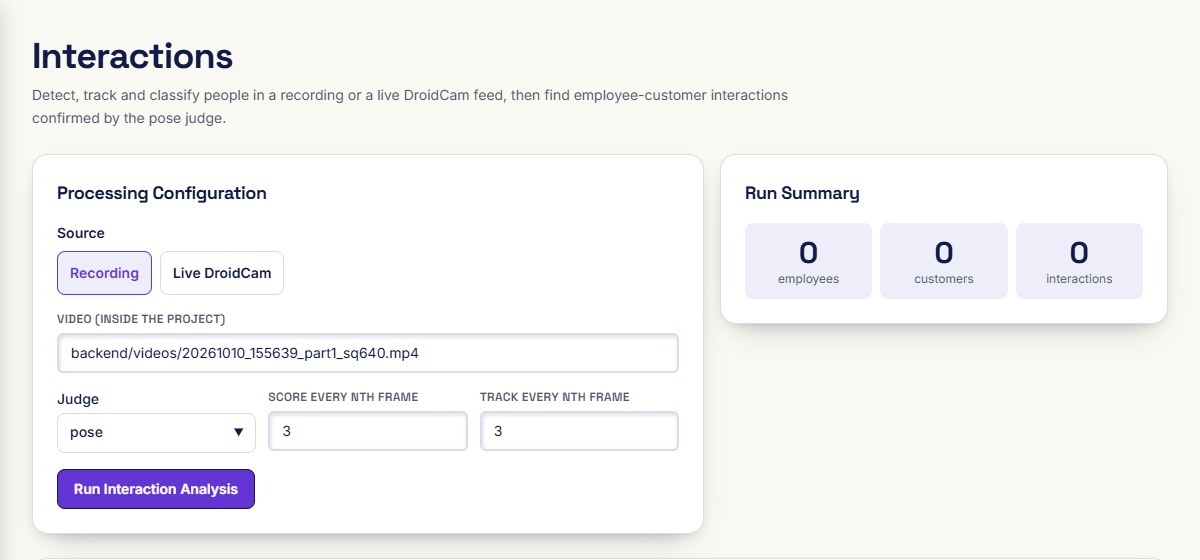
\includegraphics[width=\textwidth]{ThesisFigs/ui_interactions.png}
\caption[Interaction analysis page]{Interaction analysis page, where the manager starts a run on a recording or a live camera with the pose judge and sampling rates (UC-02).}
\label{fig:ui-interactions}
\end{figure}

\begin{figure}[htbp]
\centering
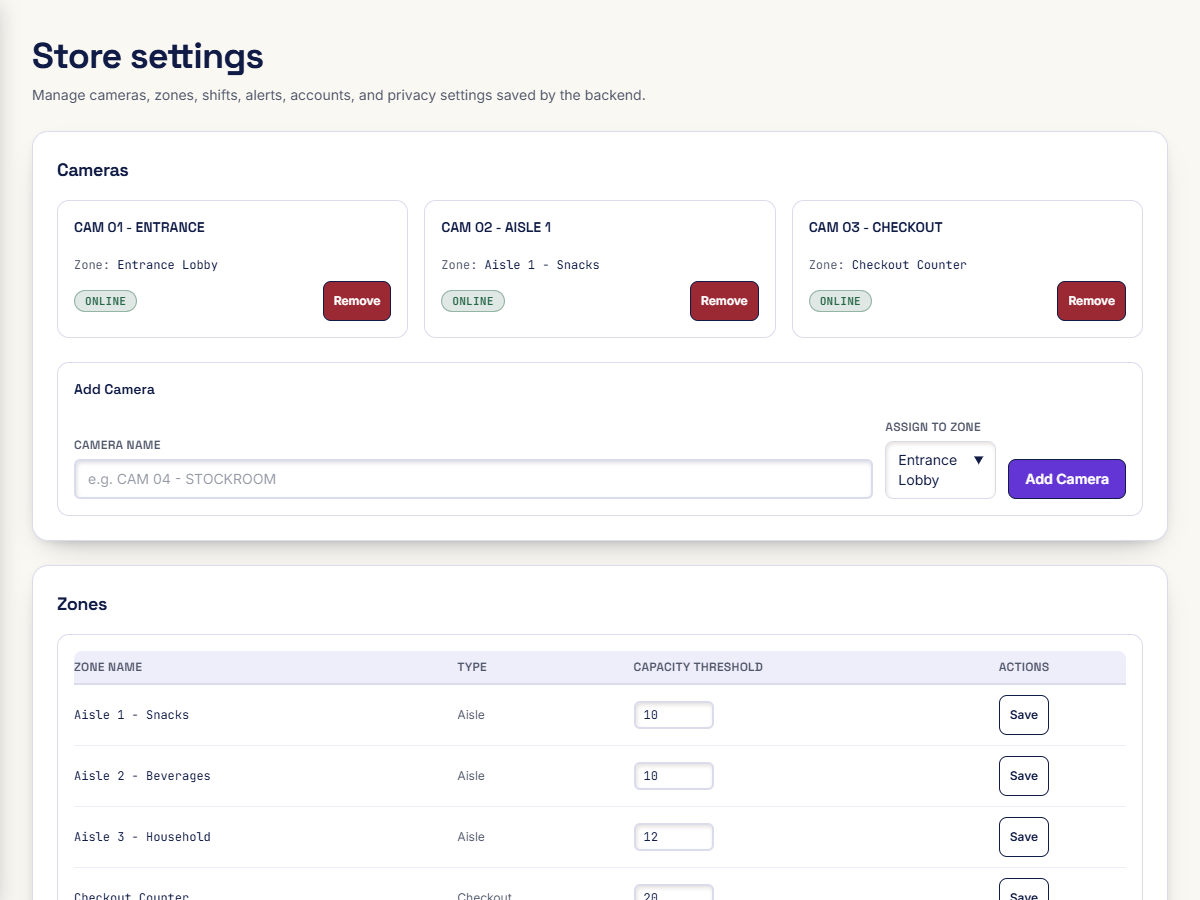
\includegraphics[width=\textwidth]{ThesisFigs/ui_settings.png}
\caption[Store settings]{Store settings for cameras and zones, saved by the backend (FR-31).}
\label{fig:ui-settings}
\end{figure}
